\section{Row matrices and polynomial vacua}\label{c01-c1-the-row-matrices-and-two-fusions}

The algebra has two outputs. Commuting transfer rows and their simple
physical eigenline will supply the boundary susceptibility in
Section~\ref{c01-c1-the-boundary-exponent}. A polynomial representative
of that eigenline will supply the polygon pairing. We first establish
the local relations that both constructions use.

The rhombus weights are the dilute-loop weights of
\cite[Eq.~(1.2)]{ZhouBatchelor1997}, divided by the empty weight.
Related dilute Yang--Baxter operators admit the two-colour braid--monoid
formulation of Grimm and Pearce~\cite[Sections~4.2, 4.5--4.6]{GrimmPearce1993}.
We specify the gauge here and verify the local and transfer identities
needed below.

\subsection*{The checked tile and its rank reductions}

Write \(q=e^{i\lambda},\ t=q^2,\ T=t^3,\ V=\mathbb C^{\{0,+1,-1\}}\).
We denote standard tensors by lists of spins in kets. The charge of a
tensor is the sum of its spins. Transpose throughout this construction
involves no conjugation. Put \(n_0=\sqrt2-1\) and define a vector \(C\)
and a map \(I:V\to V^{\otimes2}\), whose columns are \(I_h\):
\[
 C=|00\rangle+\sum_{h=\pm1}q^{5h}|h,-h\rangle,\quad
 I_0=|00\rangle+x_*\sum_{h=\pm1}q^{4h}|h,-h\rangle,\quad
 I_h=x_*(q^h|h,0\rangle+q^{-h}|0,h\rangle).
\]
Direct multiplication gives
\[
 I^tI=n_0\,1_V,\qquad C^tC=-n_0,\qquad C^tI=0.
\]
Thus \(P_1=II^t/n_0,\ P_0=-CC^t/n_0,\ P_2=1-P_1-P_0\)
are mutually orthogonal idempotents for this bilinear form. The
\emph{checked} matrix is
\[
 F(z)=\sum_{j=0}^2 r_j(z)P_j,\qquad
 (r_0,r_1,r_2)=(a,b,ab),\quad
 a=\frac{t^2-z}{t^2z-1},\quad b=\frac{T-z}{Tz-1}.
\]
It acts between ordered tensor slots of parameters \(u,w\) with \(z=u/w\),
and outputs in order \(w,u\). It preserves charge, is symmetric, and satisfies
\[
 F(1)=1,\qquad F(z)F(1/z)=1,\qquad
 F(T)=CC^t=-n_0P_0,\qquad F(t^2)=II^t=n_0P_1.
\]
The last two specializations reduce two spin slots to a cup, or to one
spin slot embedded by \(I\).

Here is its geometric realization. On a rhombus of angle \(\theta\) (bottom edge to side at the left, counterclockwise), set \(v=3\theta/8,\ z=e^{2iv}\), \(D=\sin(2\lambda+v)\sin(3\lambda+v)\). Allowed unoriented pieces have these weights:
\par\noindent\textbullet\quad empty 1; a single arc joining right to top or left to bottom has weight \(u_1=\sin(2\lambda)\sin(3\lambda-v)/D\);
\par\noindent\textbullet\quad a single arc round either other corner has weight \(u_2=\sin(2\lambda)\sin v/D\); opposite-edge connection \(o=\sin(3\lambda-v)\sin v/D\);
\par\noindent\textbullet\quad a pair of disjoint arcs at the first two corners has weight \(w_1=\sin(3\lambda-v)\sin(2\lambda-v)/D\); at the other two, \(w_2=\sin(v-\lambda)\sin v/D\).

Orient all arcs, giving them the phase \(e^{\mathrm i W/4}\) for their turns (normal incidence, turns in \((-\pi,\pi)\)). Horizontal-stream labels are \(i,k\) at right, left respectively (+ pointing leftwards across), vertical-stream \(j,l\) at bottom, top (+ towards top); vacant means 0. Multiply by the further (gauge) factor \(e^{5\mathrm i v(i-k)/3}=e^{5\mathrm i v(l-j)/3}\). The resulting sum is \(F(z)_{l k,i j}\). Indeed the blocks on \((|h0\rangle,|0h\rangle)\) have diagonals \(u_1 e^{\mathrm i hv},u_1 e^{-\mathrm i hv}\) and off-diagonal \(o\); on \(|00\rangle,|+,-\rangle,|-,+\rangle\) the matrix is symmetric, first diagonal 1, the couplings to \(|h,-h\rangle\) are \(u_2 q^{2h}e^{\mathrm i hv}\), the latter diagonals \((w_1+t^{2h}w_2)e^{2\mathrm i hv}\), and their mutual coupling \(w_2\); on charge \(\pm2\) it is \(w_1\). These entries also follow by substituting \(r_j\) above (\(a,b=\sin(k\lambda-v)/\sin(k\lambda+v)\), \(k=2,3\), giving
\(F=w_1\,1+x_*^{-2} o II^t-x_*^{-1}\sin(2\lambda-v)\sin v\, CC^t/D\)). At \(v=\lambda\) the rhombus splits into two triangles and \(u_1=x_*,\ u_2=o=w_1=x_*^2,\ w_2=0\), exactly giving the disjoint honeycomb paths. Reflection gives the corresponding realization at \(v=2\lambda\). From the same entries the matrix at \(z=0\) has \(k\ge i\), at \(z=\infty\) has \(k\le i\). Its diagonal in stream order (\(k=i,l=j\)) at 0 has value 1 if either spin vanishes, \(t^5\) if they are equal nonzero, \(t^3\) if opposite nonzero; at infinity the inverse values.

\begin{figure}[tb]
\centering
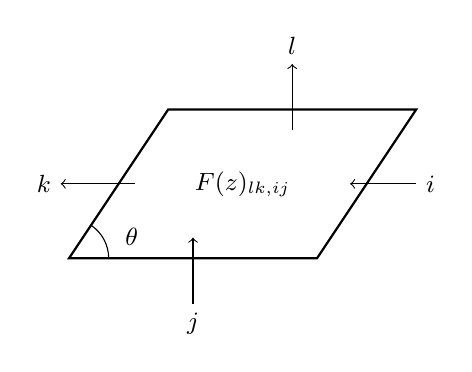
\begin{tikzpicture}[scale=1.05,every node/.style={font=\small}]
 \draw[thick] (0,0)--(3,0)--(4.2,1.8)--(1.2,1.8)--cycle;
 \draw[->] (4.2,.9)--(3.4,.9);
 \draw[->] (.8,.9)--(-.1,.9);
 \draw[->] (1.5,-.55)--(1.5,.25);
 \draw[->] (2.7,1.55)--(2.7,2.35);
 \node[right] at (4.2,.9) {$i$};
 \node[left] at (-.1,.9) {$k$};
 \node[below] at (1.5,-.55) {$j$};
 \node[above] at (2.7,2.35) {$l$};
 \draw (.48,0) arc[start angle=0,end angle=56.31,radius=.48];
 \node at (.76,.26) {$\theta$};
 \node at (2.1,.9) {$F(z)_{lk,ij}$};
\end{tikzpicture}
\caption{Port and tensor order for the checked rhombus matrix.
The horizontal stream enters at the right and leaves at the left;
the vertical stream enters below and leaves above. The arrows specify
the positive spin directions, not a particular allowed path pairing.
The local phase convention is imposed on each pairing separately.}
\label{fig:pv:row}
\end{figure}


For any of the nondegenerate real rhombi used geometrically the allowed pairings can indeed be drawn disjointly with these turns: perturb straight chords between ports by giving them short inward-normal segments at their endpoints (the chord points strictly into the first supporting line's half-plane and out towards the last line, so the two direction changes each have magnitude \(<\pi/2\)). In the two-triangle case the actual honeycomb connections have the same turns.

\begin{lemma}[Local slide and interchange relations]\label{lem:pv:local-relations}
As rational identities, the maps from \(V\) and \(V^{\otimes2}\), respectively,
to \(V^{\otimes3}\) satisfy
\[
 F_{12}(z)F_{23}(Tz)(C\otimes1)=1\otimes C,\qquad
 F_{12}(z)F_{23}(t^2 z)(I\otimes1)=(1\otimes I)F(tz).
\]
The checked matrices also satisfy the Yang--Baxter equation
\[
 F_{12}(y)F_{23}(zy)F_{12}(z)
 =F_{23}(z)F_{12}(zy)F_{23}(y).
\]
\end{lemma}

\begin{proof}
We first prove the slides by projecting onto the three channels. Write
\(m=(1,1+1/\sqrt2,1/\sqrt2)\), \(c=(1/n_0,\sqrt2,2+\sqrt2)\).
The needed small contractions are
\[
 (1\otimes C^t)(C\otimes1)=1,\quad
 (1\otimes C^t)(I\otimes1)=(C^t\otimes1)(1\otimes I)=I^t,\quad
 (1\otimes I)C=(I\otimes1)C,
\]
\[
 (1\otimes I^t)(I\otimes1)/n_0=\sum m_j P_j,\qquad
 1\otimes C-C\otimes1=(2+\sqrt2)(1\otimes I-I\otimes1)I.
\]
All are direct products of the tensors above; e.g. one can use \(C_{ab}=\delta_{a,-b}q^{5a}\) and \(I_{ab,h}=\delta_{h,a+b}J(a,b)\), with \(J(0,0)=1, J(h,-h)=x_*q^{4h},J(h,0)=x_*q^h,J(0,h)=x_*q^{-h}\) for \(h\ne0\) (invalid labels zero); the last identity reads
\[
 \delta_{ah} C_{bc}-C_{ab}\delta_{ch}
 =x_*^{-2}\delta_{a+b+c,h}
 [J(b,c)J(a,b+c)-J(a,b)J(a+b,c)] .
\]
Similarly \((1\otimes I^t)(I\otimes1)=x_*^2(1-CC^t)+II^t\) reduces entrywise at \(a+k=h+c\) to
\[
 J(a,h-a)J(h-a,c)=x_*^2(\delta_{ah}-\delta_{h,-c}q^{5(a+h)})+J(a,k)J(h,c),
\]
using \(q^8=-1,\ q+q^{-1}=x_*^{-1}\).
Consequently \(P_{j,12}(1\otimes C)=c_j P_{j,12}(1\otimes I)I\) (first project onto 0 and 1, then subtract). Project the first slide onto \(P_{j,12}\); the scalar required, relative to its right side, is
\[
 r_j(z)\big[-\delta_{j0}n_0 r_2(Tz)
 -(r_0-r_2)(Tz)/n_0+(r_1-r_2)(Tz)/(n_0 c_j)\big]=1 .
\]
For the second slide sandwich between \(P_{j,12}\) and \(P_k\) on the source. Relative to \(P_{j,12}(1\otimes I)P_k\) the multipliers on the two sides are
\[
 r_j(z)\big[\delta_{j1}r_2(t^2 z)/m_k-\delta_{k1}c_j (r_0-r_2)(t^2 z)+m_k(r_1-r_2)(t^2 z)\big]=r_k(tz)
\]
whenever \(j=1\) or \(k=1\) or \(j=k=2\). The scalar equalities are substitutions of \(a,b\) above: with \(p=t^2\) use the common denominator \((pu-1)(Tu-1)\) for \((r_2,r_0-r_2,r_1-r_2)(u)\), with numerators \((p-u)(T-u),(p-u)(T+1)(u-1),(T-u)(p+1)(u-1)\). At \(u=Tz,pz\) the denominators are \(T(p-z)(T-z),(1+z)(1+tz)\) respectively; \(a(tz)=(p-tz)/(Tz-1)\), \(b(tz)=-(T-tz)/(z+1)\). In the remaining cases the tensor factor vanishes by the contractions. This proves the slides. Inverse and transpose slides follow as well, using unitarity as rational identities.

Explicitly, denoting the three numerators just given by \(D_2,D_0',D_1'\), expansion using \(p^2=-1,\ t=(1+p)/\sqrt2,\ T=(p-1)/\sqrt2\) reads (indices ordered \(0,1,2\))
\[
 \left[-\delta_{j0}n_0 D_2-D'_0/n_0+D'_1/(n_0 c_j)\right](Tz)
 =T\begin{pmatrix}(T-z)(p z-1)\\(p-z)(Tz-1)\\(p z-1)(Tz-1)\end{pmatrix}_j ,
\]
{\small
\[
 \left[\delta_{j1}D_2/m_k-\delta_{k1}c_j D'_0+m_k D'_1\right](pz)
 =
 \begin{pmatrix}
 * & -t(1+tz)(p z-1)&*\\
 -p(1+z)(t-z)&p(p-z)(Tz-1)&T(p-z)(t-z)\\
 * &p(p z-1)(Tz-1)&T(t-z)(p z-1)
 \end{pmatrix}_{j k}
\]
}
where \(*\) entries are not needed.

For Yang--Baxter, clear the denominators and interpolate in \(z\).
For this use of degeneration values in dilute-loop Yang--Baxter
relations, compare~\cite[Section~4]{MorinDuchesnePearce2019}.
Both sides have degree at most four, and for generic \(y\) the five
points
\[
 1,\quad T,\quad t^2,\quad T/y,\quad t^2/y
\]
are distinct. Equality at \(z=1\) is immediate. At \(z=T,t^2\), the
\(z\) factor is \(EE^t\), with \(E=C,I\), respectively; sliding \(E\)
on the left and \(E^t\) on the right gives equality. Here the
reversed-order slide before transposing is the inverse slide at
\(1/(zy)\). The cases \(zy=T,t^2\) follow from the preceding cases
at \((zy,1/y)\) by unitarity. This proves the rational identity.
\end{proof}

\subsection*{Twisted rows and the physical eigenline}

For \(X=(x_1,\ldots,x_N)\) and \(\kappa\ne0\), bring an auxiliary
slot of parameter \(z\) past the sites in their listed order and trace
its output against its input, weighting the identified spin \(h\) by
\(\kappa^h\). This defines the row transfer
\(\mathcal T_\kappa(z;X)\) on \(V^{\otimes N}\). Explicitly, for
input spins \(j_1,\ldots,j_N\) and output spins \(l_1,\ldots,l_N\),
\[
 [\mathcal T_\kappa(z;X)]_{\boldsymbol l,\boldsymbol j}
 =\sum_{i_0,\ldots,i_{N-1}\in\{0,\pm1\}}
 \kappa^{i_0}\prod_{a=1}^N
 F(z/x_a)_{l_a i_a,i_{a-1}j_a},\qquad i_N=i_0.
\]
Thus site order follows the horizontal auxiliary stream, from right to
left in the tile convention of Figure~\ref{fig:pv:row}.

\begin{lemma}[Row relations]\label{lem:pv:row-relations}
At fixed twist, the row transfers commute in their row arguments.
Exchanging adjacent sites by \(F\) intertwines the corresponding rows.
At generic sites, and hence meromorphically,
\[
 \mathcal T_{\kappa}(x_j)\mathcal T_{\kappa}(Tx_j)=1,\qquad
 \mathcal T_{\kappa}(x_j)\mathcal T_{\kappa}(t^2x_j)=\mathcal T_{\kappa}(tx_j).
\]
For adjacent sites \((x,Tx)\), insertion of \(C\) intertwines the row
with the row omitting those sites. For \((x,t^2x)\), insertion of \(I\)
intertwines it with the row having the single site \(tx\). On charge zero,
\(\mathcal T_\kappa(0)=(1+\kappa+\kappa^{-1})1\).
\end{lemma}

\begin{proof}
For commutation, insert a generic invertible crossing of two auxiliary
lines, move it through the sites by Yang--Baxter, and remove it in the
trace; charge conservation preserves the product twist. The same
identity intertwines a site exchange.

For the two row fusion identities, take the indicated auxiliary pair
in that order. The second auxiliary crosses each site first. The slide
preserves its embedded \(C\) or \(I\) subspace throughout, and at the
site \(x_j\) the rank reduction followed by a checked identity sends
the whole auxiliary space into that subspace. The twisted trace is
therefore the fused trace: the product twist on \(C\) is 1, and on
the \(I\) image it is the single twist under the identification.
The inverse slides give the corresponding statements for a pair of
sites. Finally, at row argument zero, triangularity forces the auxiliary
spin to remain constant around the trace. The stated diagonal values
of \(F(0)\), together with charge zero, give
\(1+\kappa+\kappa^{-1}\).
\end{proof}

\begin{lemma}[Physical eigenline]\label{lem:pv:physical-eigenline}
At \(X=(1,\ldots,1)\), \(z=t\), and \(\kappa=\pm i\), powers of
the row transfer converge exponentially to a rank-one projection whose
empty-to-empty entry is 1. In particular, eigenvalue 1 is simple and
all other eigenvalues have modulus less than 1. The same conclusions
hold at the reflected honeycomb point \(z=t^2\).

Near either set of physical sites and twist, the rows have a common
analytic eigenline of charge zero. Its eigenvalue is rational in the
row argument and analytic in the other data near regular arguments.
At \(\kappa=\pm i\) this row eigenvalue is identically 1.
\end{lemma}

\begin{proof}
The empty basis tensor has all spins zero. At the homogeneous point,
closed loops cancel after orientation summation: contractible loops
have turns \(\pm2\pi\), with trace twist net 1, while simple essential
loops have winding \(\pm1\), trace twist \(\kappa^{\pm1}\), and total
turn zero. The latter total turn follows from the exterior-angle sum
on the annular region between the curve and a distant parallel geodesic,
which is zero by triangulation and Euler's formula. The winding assertion
also follows by identifying the cylinder with a punctured plane. Gauge
factors telescope, so only prescribed boundary-to-boundary arcs remain.

At least one crossing arc gives an exponentially small contribution
by the finite-width cylinder bounds in Lemma~\ref{lem:pv:cylinder-decay}.
With no crossing arc,
the systems along the two cuts factor in the limit into half-cylinder
amplitudes. Their error is exponentially small, since a system preventing
factorization must reach halfway across the cylinder height. There are
only finitely many boundary pairings and orientations, and dropping
mutual avoidance bounds each of them by products of arc weights. This
gives the rank-one limit. Its empty-to-empty entry is 1 because every
nonempty closed system cancels already at finite height. Reflection
gives the same argument at the other honeycomb realization.

Finite-dimensional perturbation of \(\mathcal T_\kappa(t)\) now gives
a simple analytic eigenline near the physical data. Commutation makes
it a common eigenline, and charge conservation keeps it in charge zero.
For fixed sites and twist its row eigenvalue is rational in \(z\).

To identify this eigenvalue at \(\kappa=\pm i\), first take real nearby
spectral angles \(z=e^{2iu},x_j=e^{2i\alpha_j}\). Lay the rows using
unit rhombus side vectors with directions \(8u/3\) and bottom vectors
with directions \(8\alpha_j/3\). The slightly zigzag spatial boundary
repeats by translation and projects monotonically onto the direction
perpendicular to the row side vector, so the rows do not overlap.
Loop turns and twists still cancel. The gauge factors telescope because
\(v=u-\alpha_j\) and \(i-k=l-j_{\rm spin}\) at every crossing: the
\(u\) term sums along auxiliary strands and the site-angle term along
site strands. Hence every empty-to-empty power remains 1.

Analyticity extends this equality to complex nearby data. With \(z\)
also near \(t\), all other eigenvalues remain strictly inside the unit
disk and the empty entry of the near-1 projection is nonzero. The
constant power entry therefore forces the distinguished eigenvalue
and that projection entry to equal 1. Rational continuation in \(z\)
finishes the proof.
\end{proof}
